\chapter{Constructing Trees from Lassos}
\label{cha:lasso-construction}

\textit{\sffamily This chapter is largely based on an early version of the
  following paper:}

\vspace{0.5em}

\noindent
\bibentry{kettleborough15lasso}

% \begin{itemize}
% \item George Kettleborough, Jo Dicks, Ian N. Roberts, and Katharina T. Huber.
%   Reconstructing (super)trees from data sets with missing distances: Not all
%   is lost (submitted).
% \end{itemize}

\begin{center}
  \Pisymbol{MinionPro-Extra}{121}
\end{center}

\textit{\sffamily I developed the \textsc{Lasso} algorithm and the simulation
  study for testing it.  I was also responsible for processing the biological
  datasets and using them for testing.  This involved implementation of the
  algorithm and methods described.  I also implemented the methods for drawing
  the phylogenetic trees found in the chapter.}

\newpage

\section{Introduction}
\label{sec:introduction}

\subsection{Summary}

\textsc{In this chapter} we introduce a new algorithm for reconstructing an
equidistant $X$-tree from a partial distance on $X$.  The algorithm returns
both an $X$-tree and a subset of the distances given which correspond to an
equidistant lasso for the $X$-tree.  To understand the performance of
\textsc{Lasso}, we assess it by means of artificial and real biological
datasets, showing its effectiveness in the presence of missing data even in
the presence of noise.  We also show how it can be applied to the problem of
combining datasets to build a supertree and compare our method with a well
known supertree method.

\subsection{Motivation}
\label{sec:lasso-motivation}

The ease and speed with which molecular sequence data can now be generated
using modern Next Generation Sequencing (NGS) technologies has enabled
evolutionary biologists to embark on exciting, albeit highly challenging,
endeavours such as the Tree of Life project. NGS has perhaps been most
influential at the sub-species level, and datasets encompassing numerous
lines, strains or accessions are becoming commonplace. These new data,
together with a wealth of legacy datasets, promise the interleaving of species
and sub-species within a common evolutionary framework.  However, to increase
our chances of successfully constructing such a tree numerous obstacles have
to be overcome, ranging from data collection via data storage and information
extraction to tree building. The vastness of tree space one faces in
overcoming the latter obstacle, that of tree building, coupled with the
computational demands of Bayesian, likelihood and parsimony approaches implies
that reconstruction methods based on these approaches cannot, at least at
present, be directly applied to obtain such a tree. Given the large amount of
legacy phylogenetic data, a natural solution is to try to find ways to merge
what is already known and then to augment the result. Apart from having to
deal with the problem of patchy taxonomic coverage, as some taxa have been
studied more than others (see, for example,
\cite{sanderson10phylogenomics,philippe2004phylogenomics,steel10characterizing,roure12impact}
for more on this), constructing such a tree does not only entail finding ways
to combine different types, qualities, and quantities of data but also
addresses the problem of how to combine data sets that might only share very
few taxa. The latter is a formidable problem in its own right and boils down
to finding powerful ways of dealing with missing information.

Depending on the study within which a dataset was generated missing
information may take the form of trees that have few taxa in common, or
missing values in character state or distance matrices.  To tackle the former,
numerous supertree approaches have been introduced in the literature (see, for
example, \cite{bininda04phylogenetic} and \cite{brinkmeyer13flipcut} and the
references therein).  A similar number of supermatrix approaches have also
been proposed to deal with missing values in character state matrices (see,
for example, \cite{bininda04phylogenetic}) while the number of approaches
addressing missing values in distance matrices is comparatively small (see
\cite{criscuolo2006sdm,criscuolo2008fastnj,makarenkov2001nouvelle,guenoche1999approximations,guenoche2004extension,de1984ultrametric,gaul1994pyramidal}).

The starting point for many supertree approaches is a collection of
(potentially very small) phylogenetic trees and the goal is to find some kind
of parental tree on all the taxa of the input trees that in some sense
displays the evolutionary information contained within them.  In contrast, the
starting point for the remaining two approaches are character state matrices
and distances on differing taxa sets, respectively. The aim here is to combine
them into a supermatrix or distance, respectively, on all the taxa in the
combined taxa set using some sort of imputing scheme (see
e.\,g\,\cite{bininda04phylogenetic} and \cite{queiroz06supermatrix} for such
schemes in the supermatrix context and
\cite{guenoche1999approximations,makarenkov2001nouvelle,guenoche2004extension}
in the distance context).  From the obtained matrices a phylogenetic tree is
then constructed using one of the many tree reconstruction techniques.

All three types of approach have their pros and cons, with supermatrices being
criticised on, for example, the dependence of the generated supermatrix upon
the order in which the missing values are inferred, and the potentially heavy
influence of even a small error in the estimation of a missing value on the
tree topology, the latter due to a cascading effect such an error might have
on other inferred missing values \cite{lapointe04everything}.  Criticisms of
supertrees include not using primary information, combining trees that have
potentially evolved under different evolutionary models into a supertree
without properly accounting for this, and not properly taking branch-lengths
associated with the input trees into account (see \cite{willson04constructing}
for an exception to this and \cite{kupczok11consequences} for a recent
comparison of supertree methods).  Finally, criticisms of distances include
losing valuable phylogenetic information between, for example, two DNA
sequences by representing the observed difference by a single number.
Nonetheless, distance-based tree reconstruction methods are known to provide
quick but rough snapshots of the evolutionary relationships contained within a
dataset making them particularly attractive for large datasets. In addition to
providing evolutionary insights in their own right their attraction also lies
in the provision of a potentially good starting/guide tree for more
sophisticated, but computationally intensive, methods such as Maximum
Likelihood and Bayesian Inference.

For popular distance methods such as Neighbor Joining \cite{saitou1987nj}, and
BioNJ \cite{gascuel97bionj} (in the unrooted case) and \textsc{UPGMA}
\cite{sokal1958statistical} (in the rooted case) to be applicable, however,
the distance on the combined taxa set $X$ must be complete.  As we saw in
Section~\ref{sec:constr-from-part}, it is possible to reconstruct trees from
partial distance information, but the existing algorithms deal only with the
problem of existence of a tree that fits the partial distance, they say
nothing about the uniqueness of the solution.  In this chapter we focus on the
problem of finding a unique equidistant $X$-tree for some subset of the given
distances.

From a biological point of view, equidistant $X$-trees are commonly
constructed when a molecular clock can be assumed for the evolution of the
taxa of interest.  Although molecular clocks have been criticised strongly
over the years (see \cite{ayala99molecular,schwartz06molecular}), widely-used
software packages such as BEAST rely heavily on the concept
\cite{bouckaert14beast}.  Intriguingly, this popularity may be linked in part
to the recent emergence of NGS datasets, including many consistent with a
molecular clock, particularly those at the sub-species level.  Indeed,
examples of studies where the molecular clock assumption has been satisfied
include population studies where they helped to understand the genetic
diversity of germplasms \cite{xiao10ssr}, palaeontological studies where they
helped to estimate divergence dates or shed light into effects that climate
change and other global factors might have had on diversification
\cite{weir08ice}, and phylogeographic studies \cite{confal1998mitochon} (see
\cite{weir08calibrating} for more on these examples and
\cite{hellmuth13orthology} where so called symbolic ultrametric trees were
used in orthology detection).

In the form of the \textsc{Lasso} approach, we propose a novel method for
(super)tree reconstruction from partial distances, that is, some of the
distance values between taxa are missing. Contrary to the methods alluded to
above, \textsc{Lasso} is not imputing-based and is similar in spirit to the
supermatrix approach introduced in \cite{misof13selecting} and the
veto-supertree approach proposed in \cite{scorn08physic} in that not every
taxon in the combined taxa set is guaranteed to be a leaf in the resulting
tree. It essentially works by trying to detect a treelike signal on as many
taxa as possible from the available distances and then reconstructs the
\textit{unique} equidistant tree on those taxa.  Like {\sc UPGMA},
\textsc{Lasso} is also an iterative process in the sense that it begins with a
partial (or complete) distance $D$ on some taxa set $X$ with a graph $G$ of
$|X|$ isolated vertices, each of which is labelled by an element in $X$. In
each repetition step, the distance on a smaller taxa set is recomputed and, in
a bottom up manner, an equidistant tree on $X$ is reconstructed. In contrast
to {\sc UPGMA}, \textsc{Lasso} looks to replace a certain type of
edge-weighted clique in a canonical graph theoretical representation of the
given distances by a composite vertex, rather than only an edge in that graph
as {\sc UPGMA} does. In addition, the distances between a newly created
composite vertex and any other vertices is calculated by some kind of
consensus rather than merely using average linkage as in the case of {\sc
  UPGMA}.  These two differences ensure that \textsc{Lasso} enjoys several
desirable properties such as {\em consistency} whereby we mean that the
equidistant tree $T$ returned by {\sc Lasso} is the unique tree which, for any
two taxa $x$ and $y$ in the returned lasso, the given distance $d(x,y)$ is
equal to the distance between them in $T$.

% We assessed the performance of \textsc{Lasso} as a tree reconstruction approach
% from partial distances using simulated datasets and a real biological dataset
% containing 26 intra-specific strains of the wild yeast \textit{Saccharomyces
%   paradoxus} \cite{west14ribosomal}.  In both studies, and independent of the
% shape of the topology of the starting equidistant tree, we found that even
% with $10\%$ of the distances missing \textsc{Lasso} was able to successfully
% reconstruct that tree, suggesting that it holds great promise for tree
% reconstruction in the face of missing values.  In addition, to help illustrate
% \textsc{Lasso}'s potential as a supertree approach we applied it to a wheat
% accession dataset which we obtained by combining 411 wheat accessions
% generated as part of the GEDIFLUX EU Framework V project \cite{gediflux} with
% a dataset containing 118 accessions studied in \cite{muge}, approximately a
% quarter of which are also included in the GEDIFLUX dataset. Finally, to enable
% other researchers to apply \textsc{Lasso} to their own datasets, we implemented
% the approach within software which, together with an accompanying manual, is
% freely available for download from https://www.uea.ac.uk/computing/lasso.

\section{The {\sc Lasso} algorithm}
\label{sec:sc-lasso-algorithm}

\textsc{In this section}, we present an outline of the \textsc{Lasso}
algorithm.  The algorithm is similar in spirit to \textsc{UPGMA} (as shown in
Section~\ref{sec:upgma}).  Like \textsc{UPGMA}, the \textsc{Lasso} approach is
to construct the tree from the bottom up in a repetitive fashion where each
repetition consists of a reduction step and a construction step.  However, and
contrary to {\sc UPGMA}, \textsc{Lasso} takes as input a partial distance on
$X$ (which can of course also be complete).  The complete algorithm outline is
shown in Algorithm~\ref{alg:lasso}.  In the following sections we outline the
steps in detail.

\subsection{Method outline}
\label{sec:method-outline}

Given a partial distance $D$ on some set of taxa $X$, let $\cL_D$ be the set
comprising all pairs of $X$ for which the distance under $D$ is known.

\textsc{Lasso} aims to find a subset $Y \subseteq X$ of taxa and subset $\cL'
\subseteq \cL_D$, both as large as possible, so that the equidistant tree
returned by it is uniquely determined by the available distances between pairs
in $\cL'$ with regards to topology and edge-weighting.  In other words,
\textsc{Lasso} finds an equidistant $Y$-tree $(T,\omega) $ such that the set
$\cL'$ is a strong lasso for $T$ and $D_{(T,\omega)}(x,y) =D(x,y)$ holds for
all cords $xy\in \cL'$.

To do this, $\cL_D$ is viewed as an edge-weighted graph $\Gamma_D^{\omega}$,
or $\Gamma^{\omega}$ for short. The (unweighted) underlying graph
$\Gamma(\cL_D)$ of $\Gamma^{\omega}$ has vertex set $X$ and edge set
$\cL_D$. The edge-weighting of $\Gamma^{\omega}$ associates to every edge $xy$
of $\Gamma^{\omega}$ the distance $D(x,y)$.  Note that in the case where $D$
is a complete distance on $X$, the graph $\Gamma(\cL_D)$ is complete.  To
preserve the given taxa set $X$, we put $X^r=X$.

For ease of presentation, assume from now on that we have already carried out
$q\geq 0$ repetitions and that $C$ is the selected {\em connected component}
of $\Gamma^{\omega}$, that is, one of the connected graphs that make up
$\Gamma^{\omega}$.  Note that for $q=0$ we may assume that $C$ is
$\Gamma^{\omega}$ itself as connectedness of the graph $\Gamma(\cL_D)$ and
thus of $\Gamma^{\omega}$ is a necessary condition for a $Z$-tree to be
topologically lassoed by a set of cords on some non-empty set $Z$
\cite{huber13lassoing}.  However it should be noted that $\Gamma^{\omega}$ may
become disconnected during successive repetitions.  In that case, we exploit
the fact that, as we will see below, in each repetition step an equidistant
tree is grown from (hopefully all) the vertices of a connected component of
the graph $\Gamma^{\omega}$ generated in the previous step. Put differently,
we choose a connected component of $\Gamma^{\omega}$ such that, over all
connected components of $\Gamma^{\omega}$, the leaf set of the tree grown from
it is as large as possible (where we break ties randomly). Other methods of
component choice are conceivable though, such as identifying that which
possesses the most cords of $\cL_D$.  Alternatively, it may be preferable to
run \textsc{Lasso} for each connected component of $\Gamma^{\omega}$
separately, in which case prior biological knowledge might be used to join up
the returned equidistant trees.

Note that \textsc{Lasso} terminates when the selected connected component
consists of just one vertex.  Also note that to help mitigate against a poor
choice of a connected component which might yield an equidistant tree on a
small number of taxa of $X$, \textsc{Lasso} returns the tree that connects the
most taxa in $X$ (and its associated strong lasso) found over $p$ independent
runs, where $p$ is a user defined parameter that is currently set to ten.

To simplify the description of the remaining details of the $q$-th repetition
step, let $m$ denote the minimal edge weight over all edges of $C$. Then $C$
is transformed into an unweighted graph $C_m$ in which first all edges except
those with weight $m$ have been removed and then the weights of the remaining
edges are ignored. \textsc{Lasso} now chooses a connected component $S_m$ of
$C_m$ and a {\em suitable} clique of $S_m$ (see below for details) and grows
an equidistant tree using the vertex set of that clique. To make this more
precise define for any equidistant tree $(T',\omega')$ with leaf set $Z$ the
{\em height} of $T'$ to be $D_{(T',\omega')}(x,y)/2$ for any two elements $x$
and $y$ of $Z$ for which the path joining them crosses the root of $T'$.  Let
$G$ be a graph consisting of $|X|$ isolated vertices each of which is labelled
by an element in $X$. For the purpose of growing a tree it will be useful to
view each of them as an equidistant tree with height zero.

Now, let $K_m$ denote a suitable clique of $S_m$ found by \textsc{Lasso} (where
we break ties randomly).  Then to obtain a new distance $D_m$ on a smaller set
$X_m$ which, for example, ensures that \textsc{Lasso} terminates, we first remove
all vertices in $S_m$ from $X^r$ and then add a new vertex $u_m$ to obtain
$X_m$. Next, we define $D_m$ to be the distance on $X_m$ that assigns to any
$x$ and $y$ contained in $X_m$ the value $D(x,y)$ if $x$ and $y$ in
$X_m-\{u_m\}$, zero if $x=y=u_m$ and the value $D^*(x,y)$ if either $x=u_m$ or
$y=u_m$, where $D^*$ is a distance such as the one described below in the
section on recomputing the distance $D_m$.

To find the equidistant tree $(U_m,\omega_m) $ that \textsc{Lasso} grows from $X$
in this repetition step, let $l$ denote the size of the vertex set of $K_m$
and let $(T_1,\omega_1),\ldots, (T_l,\omega_l)$ denote the equidistant trees
with leaves in $X^r$ found in the previous repetition steps such that the
vertex set of $K_m$ comprises of the roots $\rho_i$ of $T_i$, $1\leq i\leq
l$. Then to obtain $U_m$, we first add a new vertex to $G$ labelled $u_m$ and
then join every root $\rho_i$, $1\leq i\leq l$, via an edge with $u_m$ making
$U_m$ a tree with root $u_m$ and leaves contained in $X$.

To obtain the equidistant edge-weighting $\omega_m$ for $U_m$, assume for all
$i\in \{1,\ldots,l\}$ that the height $h_i$ of the tree $(T_i,\omega_i)$ was
computed in one of the previous repetition steps. Note that, by definition,
there must exist leaves $u$ and $v$ with distance $D(u,v)=m$ such that $u_m$
lies on the path from $u$ to $v$ in $U_m$. Then we define $\omega_m$ to be the
map that assigns to every edge $e$ of $U_m$ that is also contained in some
tree $T_i$, $1\leq i\leq l$, its weight under $\omega_i$ and the weight
$m/2-h_i$ if $e$ contains the root $\rho_i$, $1\leq i\leq l$. Since for all
$i\in \{1,\ldots,l\}$ the trees $(T_i,\omega_i)$ are equidistant, it is
straightforward to see that $\omega_m$ is an equidistant edge-weighting for
$U_m$ and that the height of the tree $(U_m,\omega_m) $ is $m/2$.

To complete the repetition step, we replace $X^r$ by $X_m$ and $D$ by $D_m$,
and return to finding a connected component for the new graph $\Gamma^w$ for
$D$. Once the aforementioned termination criterion is satisfied, the found
equidistant tree and its strong lasso is saved and the next run is
started. \textsc{Lasso} stops once all $p$ runs have been completed and returns
the equidistant tree and its strong lasso, as described above.

\subsection{Suitable cliques}
\label{sec:cliques}

Central to \textsc{Lasso} is finding a suitable clique in the graph
$\Gamma^{\omega}_D$ where $D$ was constructed in the previous step of the
repetition (or of the input distance if the current step is the start of the
repetition). Note that these cliques correspond to the complete graphs of
theorem~\ref{thm:child-edge-graph-complete} and give us one internal vertex.
In the case where the tree is binary these cliques are trivial (consisting of
only one edge).  To find a suitable clique, let $m$ be the minimal edge-weight
in the graph $C$ and $S_m$ a connected component with minimal edge-weight
chosen as above.  Exploiting again the fact that the new element $u_m$
constructed in the current repetition step can be thought of as the
equidistant tree $(U_m,\omega_m)$ whose leaf set is contained in $X$, we say
that a clique in $K_m$ is {\em suitable} if, over all cliques of $S_m$, the
number of taxa of $X$ it contains is as high as possible.

Since the problem of finding such a clique further requires deciding whether a
clique of a given size $K$ or more exists in a graph, and this is a well-known
NP-complete problem \cite{gareyjohnson79}, we use a heuristic for this. More
precisely, we start with a randomly chosen edge $e$ in $S_m$. Note that $e$ is
clearly a clique. Denoting that clique by $K_e$, and its vertices by $x$ and
$y$, we check for all remaining vertices $z$ of $S_m$ if they are adjacent
with every vertex of $K_e$ or not. In the former case we update $K_e$ by
adding $z$ to its vertex set and all edges of the form $\{c,z\}$ to its edge
set where $c\in K_e$, and in the latter case we discard $z$.  We continue in
this fashion until we cannot enlarge $K_e$ any further, in which case we stop
and save the found clique. To again mitigate against a poor choice, we repeat
this process $k$-times (ignoring edges that are chosen more than once) where
$k$ is a user-defined parameter that is currently set to ten. The clique that,
over all found cliques, has the largest number of leaves is the clique that we
take as the suitable clique.

\subsection{Recomputing the distance $D_m$}
\label{sec:collapsinng-edges}

\begin{figure}
  \centering
  \begin{subfigure}[b]{0.4\textwidth}
    \centering
    \begin{tikzpicture}[xscale=0.5,yscale=0.35]
      \node (r) at (0.0,0.0) {};
      \node (rr) at (-0.2,0.0) {};
      \draw (r.center) -- (rr.center);
      \node (r1) at (1.5,-2) {};
      \node[label=right:{$d$}] (r11) at (5.5,-3) {};
      \draw (r1.center) |- (r11.center);
      \node[label=right:{$c$}] (r13) at (2.5,-1) {};
      \draw (r1.center) |- (r13.center);
      \draw (r.center) |- (r1.center);
      \node (r3) at (1.0,2) {};
      \node[label=right:{$b$}] (r31) at (2.0,1) {};
      \draw (r3.center) |- (r31.center);
      \node[label=right:{$a$}] (r33) at (5.0,3) {};
      \draw (r3.center) |- (r33.center);
      \draw (r.center) |- (r3.center);
      \draw[|-|] (4.5,-4.5) -- (5.5,-4.5);
      \node at (5.0,-5.5) {1.0};
    \end{tikzpicture}
    \caption{Original tree.}
    \label{fig:non-ultrametric-tree}
  \end{subfigure}
  \begin{subfigure}[b]{0.4\textwidth}
    \centering
    \begin{tikzpicture}[xscale=0.5,yscale=0.35]
      \node (r) at (-3.85,0) {};
      \node (rr) at (-3.83,0.0) {};
      \draw (r.center) -- (rr.center);
      \node (r2) at (-3.125,1) {};
      \draw (r.center) |- (r2.center);
      \node (r22) at (-2.25,2) {};
      \draw (r2.center) |- (r22.center);
      
      \node[label=right:{$a$}] (r1) at (0,-3) {};
      \draw (r.center) |- (r1.center);
      \node[label=right:{$d$}] (r21) at (0,-1) {};
      \draw (r2.center) |- (r21.center);
      \node[label=right:{$c$}] (r221) at (0,1) {};
      \draw (r22.center) |- (r221);
      \node[label=right:{$b$}] (r222) at (0,3) {};
      \draw (r22.center) |- (r222);

      \draw[|-|] (-1,-4.5) -- (0,-4.5);
      \node at (-0.5,-5.5) {1.0};
    \end{tikzpicture}
    \caption{Tree constructed by \textsc{UPGMA}.}
    \label{fig:upgma-tree}
  \end{subfigure}
  \caption{\textsc{UPGMA} fails to reconstruct the correct tree if the
    inputted distance is not ultrametric.  Here the true (non-equidistant)
    tree is shown in (i) and the tree constructed by \textsc{UPGMA} in (ii).}
  \label{fig:upgma-fail}
\end{figure}

There are several possible choices for recomputing the distance $D_m$.
Continuing with the notation introduced above we need to define for all
vertices $a$ in $C$ but not in $S_m$ the distance $D^*(u_m,a)$ by somehow
combining the distances $D(v,a)$ for all $v$ in $K_m$.  In the straightforward
case where the inputted partial distance came from an ultrametric, the
distances $D(v,a)$ for all $a \in C$ will be equal for all $v \in K_m$.  In
this case we would simply set $D^*(u_m,a)$ to $D(v,a)$ for all $a$.  However,
in practice the distances $D(v,a)$ for some $a$ may not be equal.  There are
two reasons for this: either the partial distance does not come from an
ultrametric at all, or the data from which we derived the partial distance
information was subject to noise (as we would expect from biological data).

To illustrate this situation we consider how \textsc{UPGMA} behaves.
Figure~\ref{fig:upgma-fail}~(\ref{fig:non-ultrametric-tree}) shows an
edge-weighted $X$-tree $(T,\omega)$ with $X = \{a,\dotsc,d\}$ which is not
equidistant, therefore the induced distance $D_{(T,\omega)}$ on $X$ is not an
ultrametric.  If this distance is used as input to \textsc{UPGMA} we get the
equidistant $X$-tree $(T',\omega')$ shown in
Figure~\ref{fig:upgma-fail}~(\ref{fig:upgma-tree}).  The induced distance on
the constructed tree $D_{(T',\omega')}$ is correct only between $b$ and $c$.
To see why recall that \textsc{UPGMA} agglomerates the nearest two clusters in
each iteration, in the first iteration this is $\{b\}$ and $\{c\}$ which will
come together to form a cherry with the correct height of
$D_{(T,\omega)}(b,c)/2$.  Next the algorithm must calculate the distance
between the newly formed cluster and every other cluster using
average-linkage.  The distance between $\{b,c\}$ and $\{a\}$, for example is
calculated from the distances between $\{b\}$ and $\{a\}$ and $\{c\}$ and
$\{a\}$.  But observe that these two distances are not equal.  This is our
indication that the inputted distance was not ultrametric.

Returning to \textsc{Lasso}, it is now clear that to provide the consistency
property we cannot simply use average-linkage in the case where the distances
$D(v,a)$ are not equal.  Instead we must discard some of the input distances
such that $D(v,a)$ is equal for all $v \in K_m$ and all $a \in C - S_m$.  This
reduces the size of our outputted lasso.  To decide which of the distances to
discard the obvious way is for each $a \in C - S_m$ to take the mode of the
distances $D(v,a)$ for all $v \in K_m$ and discard those distances not equal
to the mode.  This ensures that the consistency property is satisfied while
using as many distances as possible.  The fact that the algorithm has not used
every distance in the input can be used as a sign that the inputted distance
was not ultrametric.  In the worst case, the lasso returned by the algorithm
will be only a minimal topological lasso even if many more distances were
inputted.  Indeed, this is the case if we try the example of
Figure~\ref{fig:upgma-fail} using the above procedure to calculate $D^*$.

However, this does not take into account the fact that real data is noisy.  In
practice we can rarely expect to find equality, but this does not necessarily
mean that the real underlying tree is not equidistant.  To enable tolerance to
noise we try to find for each $a \in C - S_m$ a cluster of distances in
$D(v,a)$ over all $v \in K_m$.  The distances in the cluster should be similar
to within some noise threshold.  We then discard distances not in the cluster
and set $D^*(u_m,a)$ to the mean of the distances in the cluster.

To find a single cluster we can use a simple iterative approach.  Let $S
\subset \rrnn$ be our set of distance values and $\bar{s}$ the mean of all
values in $S$.  We find an $s \in S$ such that $|s - \bar{s}|$ is maximised
and remove this value if $\sigma = |s - \bar{s}|/\bar{s}$ is greater than some
threshold $\zeta$.  We repeatedly remove values from $S$ until $\sigma$ is
below the noise threshold.  We are left with our cluster $S$.  We have found
that a good value for $\zeta$ is $0.1$.

The overall algorithm is given in as Algorithm~\ref{alg:lasso}.  The runtime
complexity of the algorithm is $O(|\cL_D|^2)$ since, in the worst case, we
replace a clique consisting of only one edge in each iteration and must
perform a linear search on the edges of $\Gamma^\omega$ to find the minimum
edge-weight in each iteration.

\begin{algorithm}
  \caption{The \textsc{Lasso} algorithm}
  \label{alg:lasso}
  \textbf{Input:} Partial distance $D$ on $X$ 

  \textbf{Output:} A subset $\cL'$ of cords of $\cL_D$ and an equidistant
  $Y$-tree $(T,\omega)$ that is strongly lassoed by $\cL'$ such that $Y$ and
  $\cL'$ are as large as possible, $Y=\bigcup_{xy\in \cL'}xy$ holds, and
  $D_{(T,\omega)}(x,y) = D(x,y)$, for all $xy \in \cL'$.

  \begin{itemize}
  \item[0.] Compute $\Gamma^{\omega} =\Gamma^{\omega}_D$ and put $q := 0$
and $X^r=X$.
  \item[1.] Choose a connected component $C$ of  $\Gamma^{\omega}$ 
such that the leaf set of the equidistant tree grown from it is as 
large as possible.  If $C$ has a single vertex, terminate 
and return that tree and the found set of cords that strongly lassos it.
  \item[2.] Put $\displaystyle m := \min_{xy \in \cL_D} D(x,y)$
and compute unweighted graph $C_m$. 
  \item[3.] Choose a connected component $S_m$ of $C_m$ and a suitable
clique $K_m$ in $S_m$.
\item[4.] Using a new vertex $u_m$ and the definition of $D^*$, put $X_m :=
  X^r - S_m \cup \{u_m\}$ and the new distance $D_m$ on $X_m$, respectively.
  \item[5.] Join $u_m$ with the roots of the equidistant trees 
whose roots correspond to the vertices of $K_m$ to obtain the tree $U_m$
and define the equidistant edge-weight $\omega_m$ such that the height of
$U_m$ is $m/2$.
  \item[6.] Put $X^r:=X_m$, $D:=D_m$, $q := q+1$ and return to step 1.
  \end{itemize}
\end{algorithm}

\subsection{An example}
\label{sec:example}

To illustrate the \textsc{Lasso} approach assume that $X=\{a,\ldots, e\}$ is a
taxa set and that $D$ is a partial distance on $X$ given in terms of the
edge-weights of the graph $\Gamma^{\omega}_D$ presented in
Figure~\ref{fig:pink-const}~(i).

\begin{figure}
  \centering
  \input{figures/lasso-construction/lasso-ex-3.pdft}
  \caption{For the partial distance $D$ on $X=\{a,\ldots, e\}$ as indicated by
    the edge-weights of the graph $\Gamma^{\omega}_D$ depicted in (i) we
    depict in (iii) the equidistant tree $(T,\omega)$ returned by \textsc{Lasso}
    and in (iv) the strong lasso found by \textsc{Lasso} for $T$. In (ii) we
    depict updated distance $D_2$ in the first repetition step of \textsc{Lasso}
    in terms of the graph $\Gamma^{\omega}_{D_2}$.}
  \label{fig:pink-const}
\end{figure}
% 
Then in the first repetition step (with $q=0$) the minimal edge-weight is 2
and the connected component $C$ chosen by \textsc{Lasso} is
$\Gamma^{\omega}_D$ itself as that graph is connected. The subgraph of $C$
with vertex set $\{a,b,c,d\}$, edge set indicated in bold and edge-weights
ignored, is $C_2$. Note that this graph coincides with the connected component
$S_2$ chosen by \textsc{Lasso} as that graph is again connected. The suitable
clique chosen by \textsc{Lasso} is the subgraph with vertex set $\{b,c,d\}$
and the three edges joining them in the form of a triangle in that figure.
The equidistant tree $(U_2,\omega_2)$ grown by \textsc{Lasso} is the subtree
of the equidistant tree depicted in Figure~\ref{fig:pink-const}~(iii) with
leaf set $\{b,c,d\}$ and edges in bold. Furthermore, the updated distance
$D_2$ on $X_2=\{u_2,e\}$ is represented in terms of the graph
$\Gamma^{\omega}_{D_2}$ displayed in Figure~\ref{fig:pink-const}~(ii) where
the tie was broken by deleting the cord $de$ and thus removing the distance
$D(d,e)$. Putting $X^r=X_2$ and $D=D_2$ completes the first repetition
step. Since $\Gamma^{\omega}_D$ is again connected and contains more than one
vertex a second repetition step is carried out. Again $C$ is the graph
$\Gamma^{\omega}_D$ itself.  The minimal weight $m$ is six and $C_6$, $S_6$
and $K_6$ all equal $\Gamma^{\omega}_D$. Then $X_6=\{u_6\}$,
$D_6(u_6,u_6)=0$. The equidistant tree $(U_6,\omega_6)$ grown is depicted in
Figure~\ref{fig:pink-const}~(iii). To complete the second repetition step we
now replace $X^r$ by $X_6$ and $D$ by $D_6$. Since the graph
$\Gamma^{\omega}_{D_6}$ is connected \textsc{Lasso} picks
$\Gamma^{\omega}_{D_6}$ as the connected component. Since
$\Gamma^{\omega}_{D_6}$ contains only the vertex $u_6$, \textsc{Lasso}
terminates. For $Y=\{b,c,d,e\}$, we picture in
Figure~\ref{fig:pink-const}~(iv) the strong lasso $\cL_Y$ found by
\textsc{Lasso} for $T$ in terms of the graph $\Gamma(\cL_Y)$.  It is possible
for \textsc{Lasso} to find smaller trees (for example we could have picked the
clique with only $a$ and $b$ in the first iteration) but after multiple runs
this tree will be found as the largest.

\section{Results and Discussion}
\label{sec:results}

\textsc{The Lasso approach} enjoys several attractive theoretical
features. These include that when given a partial distance $D$ on some taxa
set $X$, the set $\cL'$ of cords returned by \textsc{Lasso} (together with the
distances for the cords in that set) uniquely determines the topology as well
as the edge-weighting of the equidistant $X'$-tree $(T,\omega)$ returned by
{\sc Lasso}, where $X'$ is the vertex set of $\Gamma(\cL')$.  In particular,
if $D$ is such that $\cL_D$ is a topological lasso for $T$ then $X=X'$.  That
is, the leaf set of $T$ is the whole of $X$.  Moreover, if $D$ is in fact a
complete distance on $X$ and ultrametric then the distance induced by
$(T,\omega)$ on $X$ is $D$.

Due to, for example, missing data it is in general too much to hope for that
the available distances in a real biological study correspond to a topological
lasso for some equidistant tree. To assess the performance of \textsc{Lasso}
as a tree reconstruction approach with regards to this confounding factor,
while controlling key aspects of the input data, we carried out a simulation
study which is similar in spirit to the one presented in
\cite{criscuolo2008fastnj}.  To gauge the performance of \textsc{Lasso} as a
tree reconstruction approach on a real biological dataset, we applied it to a
yeast dataset \cite{west14ribosomal} recently developed from a whole genome
resequencing study \cite{liti}. We further assessed the potential of
\textsc{Lasso} as a supertree approach by combining two partially overlapping
wheat datasets, developed in distinct studies \cite{gediflux, muge}.  We start
with outlining our missing data simulation scenario.

\subsection{Missing data}
\label{sec:missing-data-disc}

To better understand how the topology of an equidistant tree affects our
ability to reconstruct it from a partial distance, we first generated three
binary $X$-trees, one of which was a balanced tree, a second a caterpillar
tree, and the third we generated using the Yule-Harding model. For this, we
took the size of $X$ to be 128.  For initial unweighted tree simulation, we
implemented the approach described in \cite[Section
2.5]{semple2003phylogenetics}.  Next, we turned each of the resulting trees
into an equidistant $X$-tree. In the balanced tree case we assigned weight one
to all edges. In the caterpillar tree case we assigned the difference in
height between two adjacent vertices to the weight of the joining edge, and in
the Yule-Harding tree case we proceeded as follows. Starting with a
Yule-Harding $X$-tree $T$, we first assign to every vertex $v$ of $T$ the
number $h(v)$ of edges on a longest path from $v$ to a leaf of $T$ below $v$,
where we put $h(v)=0$ in case $v$ is a leaf.  For $e$ an edge of $T$ joining
two vertices $u$ and $v$, we then assign $|h(u)-h(v)|$ as weight to $e$.

\begin{table}
  \centering
  \begin{tabular}{rrrrrrr}
    \toprule
    $P_{miss}$ & mean  &    min   &   max  &   meanc &    minc &   maxc\\
    \midrule
    0.0 &   0.000  &  0.000   & 0.000  & 2016.000   &  2016  &   2016\\
    1.0  &  0.000  &  0.000   & 0.000  & 2015.770   &  2014  &   2016\\
    5.0  &  0.011  &  0.000   & 0.095  & 2003.480   &  1945  &   2015\\
    10.0 &   0.029 &   0.000  &  0.190 & 1976.640  &   1814 &    2005\\
    20.0 &   0.099 &  0.000   & 0.587  & 1849.600   &   475  &   1944\\
    30.0 &   0.261 &   0.000  &  0.762 & 1445.220  &    255 &    1842\\
    \bottomrule
  \end{tabular}
  \caption{Normalised Robinson-Foulds distances for the
    balanced trees and the sizes of the supporting strong lassos.}
  \label{tab:balanced}
\end{table}

\begin{table}
  \centering
  \begin{tabular}{rrrrrrr}
    \toprule
    $P_{miss}$ &  mean  &    min &     max &    meanc &    minc &   maxc\\
    \midrule
    0.0 &   0.000  &  0.000 &   0.000 & 2016.000  &   2016  &   2016\\
    1.0 &   0.000  &  0.000 &   0.000 & 2015.760  &   2013  &   2016\\
    5.0 &   0.005  &  0.000 &   0.143 & 2007.850  &   1949  &   2016\\
    10.0&    0.024 &   0.000 &   0.270 & 1982.360 &  1869 &   2003\\
    20.0 &   0.110 &   0.000 &   0.492 & 1842.460 &    672 &   1954\\
    30.0 &   0.187 &   0.000 &   0.635 & 1670.370 &    317 &   1859\\
    \bottomrule
  \end{tabular}
  \caption{Normalised Robinson-Foulds distances for the
    Yule trees and the sizes of the supporting strong lassos.}
  \label{tab:yule}
\end{table}

\begin{table}
  \centering
  \begin{tabular}{rrrrrrr}
    \toprule
    $P_{miss}$ & mean    &  min    &  max   &  meanc  &   minc &   maxc\\
    \midrule
    0.0  &  0.000  &  0.000  &  0.000 & 2016.000  &   2016   &  2016\\
    1.0  &  0.000  &  0.000  &  0.000 & 2015.780  &   2014   &  2016\\
    5.0  &  0.000  &  0.000  &  0.000 & 2011.090  &   2003   &  2016\\
    10.0 &   0.020 &   0.000 &   1.000 & 1994.720 &   1933  &   2004\\
    20.0 &   0.040 &   0.000 &   1.000 &  1931.610 &   1864  &  1954\\
    30.0 &   0.110 &   0.000 &   1.000 &  1829.440 &   1769  &  1861\\
    \bottomrule
  \end{tabular}
  \caption{Normalised Robinson-Foulds distances for the
    caterpillar trees and the sizes of the supporting strong lassos.}
  \label{tab:caterpillar}
\end{table}

For each of these three equidistant $X$-trees, we then generated an incomplete
distance matrix from the induced (complete) distance matrix by randomly
removing a percentage $P_{miss}$ of entries, ensuring that with $\cL$ denoting
the associated set of cords the $\Gamma(\cL)$ graph remained connected. More
precisely, we generated 500 incomplete distance matrices for each of the three
equidistant $X$-tree types using the values $1\%$, $5\%$, $10\%$, $20\%$ and
$30\%$ for $P_{miss}$.  We then used the resulting $3 \times 5 \times 500$
incomplete distance matrices as input to \textsc{Lasso}. Each equidistant
$X$-tree found by \textsc{Lasso} was then compared with the respective
equidistant $X$-tree $(T',\omega')$ used to generate the underlying input
matrix. More precisely, for $Y$ denoting the leaf set of a tree $(T,\omega)$
returned by \textsc{Lasso}, we computed the Robinson-Foulds distance
\cite{robinson1981comparison} $D_{RF}(T,T'|_Y)$ between $T$ and the
restriction $T'|_Y$ of $T'$ to $Y$, that is, we counted the number of clusters
induced by $T'|_Y$ but not by $T$ and vice versa.  For each equidistant
$X$-tree type and percentage $P_{miss}$, we then averaged the obtained 500
distances using the mean. We summarise our results in
Figure~\ref{fig:rob-foulds-shapes} in terms of the {\em normalised
  Robinson-Foulds distance} $D_{RF}(T,T'|_Y)/2(|X|-1)$ between $T$ and
$T'|_Y$, that is, we divided $D_{RF}(T,T'|_Y)$ by the maximal Robinson-Foulds
distance between two $X$-trees, which is $2(|X|-1)$.
Tables~\ref{tab:balanced}, \ref{tab:yule} and \ref{tab:caterpillar} show some
simple statistical measures on the supporting strong lassos.  Mean, min and
max refer to the Robinson-Foulds distance and meanc, minc and maxc refer to
the size of the lasso.

\begin{figure}
  \centering
  \beginpgfgraphicnamed{rob-foulds-shapes}
  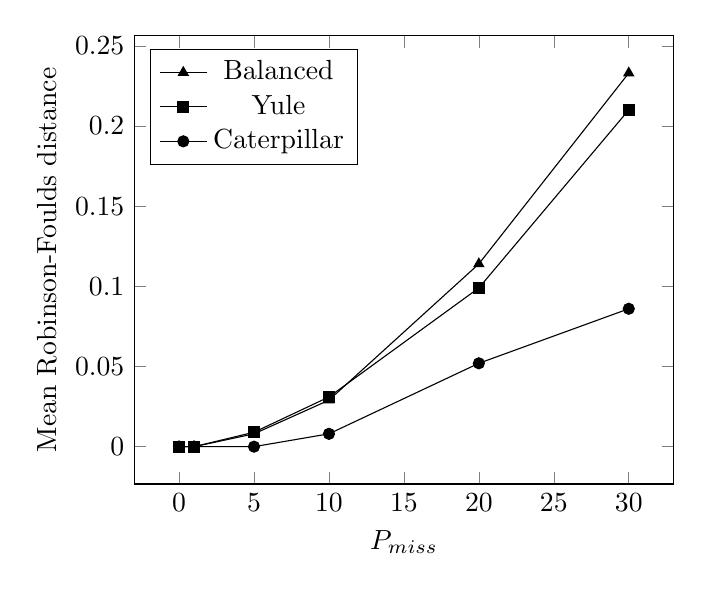
\begin{tikzpicture}
            \begin{axis}[xlabel=$P_{miss}$,
          ylabel=Mean Robinson-Foulds distance,
          yticklabels={,0,0.05,0.1,0.15,0.2,0.25},
          legend pos=north west]
      \addplot[color=black,mark=triangle*] table[x=missing,y=mean]{
missing  mean      min      max     minc     maxc
0.0    0.000    0.000    0.000       64       64
1.0    0.000    0.000    0.000       64       64
5.0    0.008    0.000    0.175       62       64
10.0    0.029    0.000    0.238       61       64
20.0    0.114    0.000    0.635       31       64
30.0    0.233    0.000    0.698       30       64
      };
      \addlegendentry{Balanced}
      \addplot[color=black,mark=square*] table[x=missing,y=mean]{
missing  mean      min      max     minc     maxc
0.0    0.000    0.000    0.000       64       64
1.0    0.000    0.000    0.000       64       64
5.0    0.009    0.000    0.206       62       64
10.0    0.031    0.000    0.397       49       64
20.0    0.099    0.000    0.619       29       64
30.0    0.210    0.000    0.857       14       64
      };
      \addlegendentry{Yule}
      \addplot[color=black,mark=*] table[x=missing,y=mean]{
missing  mean      min      max     minc     maxc
0.0    0.000    0.000    0.000       64       64
1.0    0.000    0.000    0.000       64       64
5.0    0.000    0.000    0.000       64       64
10.0    0.008    0.000    1.000       63       64
20.0    0.052    0.000    1.000       62       64
30.0    0.086    0.000    1.000       62       64
      };
      \addlegendentry{Caterpillar}
    \end{axis}

  \end{tikzpicture}
  \endpgfgraphicnamed  
  \caption{For all three equidistant $X$-tree types, we plot the normalised
    Robinson-Foulds distance between $T$ and $T'|_Y$.}
  \label{fig:rob-foulds-shapes}
\end{figure}

\begin{figure}
  \centering
  \beginpgfgraphicnamed{simulation-nleaves}
  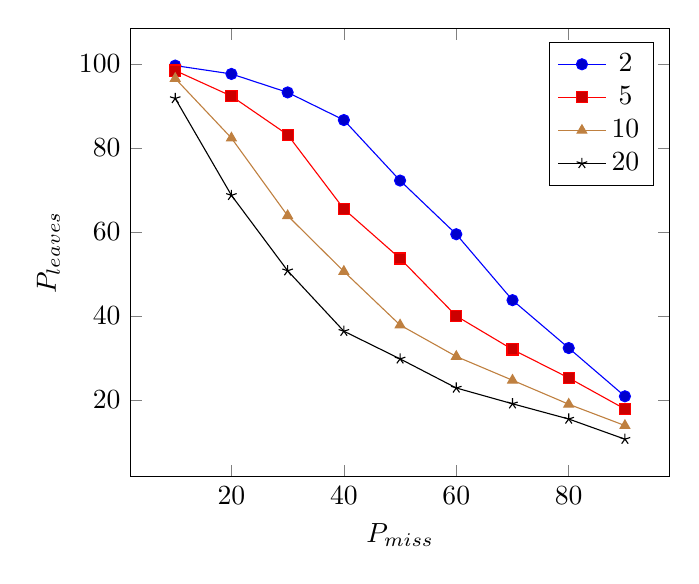
\begin{tikzpicture}
        \begin{axis}[ xlabel=$P_{miss}$,
      ylabel=$P_{leaves}$,
      legend pos=north east]

      \addplot table[x=mcords,y=nleaves] {
 mcords  nleaves   ncords
  10.00    99.64    99.53
  20.00    97.65    94.95
  30.00    93.25    88.97
  40.00    86.67    77.56
  50.00    72.26    56.96
  60.00    59.48    39.49
  70.00    43.78    22.29
  80.00    32.38    12.63
  90.00    20.89     6.47
   };
   \addlegendentry{2}
      \addplot table[x=mcords,y=nleaves] {
 mcords  nleaves   ncords
  10.00    98.46    96.99
  20.00    92.37    86.98
  30.00    83.17    71.69
  40.00    65.50    47.52
  50.00    53.70    32.66
  60.00    40.01    18.88
  70.00    32.04    12.24
  80.00    25.27     8.50
  90.00    17.86     5.54
   };
   \addlegendentry{5}
      \addplot[mark=triangle*,color=brown] table[x=mcords,y=nleaves] {
 mcords  nleaves   ncords
  10.00    96.57    93.85
  20.00    82.38    71.98
  30.00    63.89    46.22
  40.00    50.62    30.73
  50.00    37.86    17.49
  60.00    30.37    11.50
  70.00    24.71     7.92
  80.00    19.00     5.27
  90.00    13.92     3.85
   };
   \addlegendentry{10}
      \addplot table[x=mcords,y=nleaves] {
 mcords  nleaves   ncords
  10.00    91.81    86.00
  20.00    68.75    53.41
  30.00    50.79    30.61
  40.00    36.39    17.35
  50.00    29.80    11.57
  60.00    22.87     7.10
  70.00    19.11     5.28
  80.00    15.48     3.87
  90.00    10.68     2.70
   };
   \addlegendentry{20}
    \end{axis}

  \end{tikzpicture}
  \endpgfgraphicnamed  
  \caption{For $T'$ an $X$-tree with $|X|=100$ and maximum out-degree $k= 2$,
    $5$, $10$ and $20$ we depict the proportion of $X$ which forms the leaf
    set of $T$. -- see text for details.  }
  \label{fig:simulation-nleaves}
\end{figure}

We observed that, independent of the type of equidistant tree considered, the
Robinson-Foulds distance between $T'|_Y$ and $T$ increases as the number of
distance values decreases, which is as expected. Having said that, out of all
three $X$-tree types equidistant caterpillar trees were reconstructed most
accurately with a mean normalised Robinson-Foulds distance below 0.1 even when
$30\%$ of the distance values were missing. A potential reason for this might
be that to correctly reconstruct a internal vertex $v$ of $T'$ the child-edge
graph associated to $v$ must be a complete graph (see
Section~\ref{sec:lassoing-rooted-x}).  In a caterpillar tree there is only one
cherry, all other internal vertices have a child that is a tree.  So the
likelihood that the child-edge graph associated to an internal vertex is a
complete graph is high as an edge in that vertex's child edge graph tends to
be supported by many leaf pairs of $T$ implying that \textsc{Lasso} correctly
reconstructs $v$. On the other hand, a balanced tree has the highest number of
cherries. Thus, the likelihood that the child-edge graph associated to such
vertices is not a complete graph increases as the number of missing distance
values grows, implying that $T$ may be very different from $T'|_Y$. Given that
it is well-known that trees generated under the Yule-Harding model tend to be
highly balanced (see e.\,g.\,\cite[Section 2.5]{semple2003phylogenetics}) it
is unsurprising to see that equidistant Yule-Harding trees and equidistant
balanced trees exhibit a similar behaviour.  Interestingly, equidistant
Yule-Harding trees were reconstructed slightly more accurately than
equidistant balanced trees overall, presumably due to small departures from a
purely balanced state.

\begin{algorithm}[h!]
  \caption{Random tree generation}
  \label{alg:random-tree}
  \textbf{Input:} A set $X$ and an integer $k$.
  
  \textbf{Output:} An equidistant $X$-tree with maximum
  out-degree $k$.

  \begin{itemize}
  \item[1.] Choose an integer 
$p$ in $\{2, \dotsc, \min(|X|,k)\}$ and some subset $C$ of $X$ of size $p$.
  \item[2.] Construct a tree $T$ with root $\rho_T$ by
attaching each element $c$ in $C$ via an edge to $\rho_T$ 
and setting the weight of that edge to $ 1+ \max_{x \in X} \, height(x)
- height(c)$.
  \item[3.] Put $X := (X - C) \cup \{\rho_T\}$.
  \item[4.] If $|X| > 1$ go to step 1, otherwise return $T$ 
%where $X = \{T\}$.
    and its edge-weighting.
  \end{itemize}
\end{algorithm}

Figure~\ref{fig:rob-foulds-shapes} suggests that for low quantities of missing
distances, \textsc{Lasso} is very good at exploiting redundancy in a given
distance matrix to correctly reconstruct the underlying equidistant $X$-tree,
independent of the tree type. To better understand how much this observation
is dependent on the fact that the starting $X$-trees were all binary, we also
investigated the influence of the maximal vertex degree $k$ of such a tree on
\textsc{Lasso}'s performance. To this end, we generated $500$ random
equidistant $X$-trees $(T',\omega')$ with maximum vertex out-degree $k$ as
described in Algorithm~\ref{alg:random-tree}.  The values for $k$ that we used
in this study were $k=2$, $5$, $10$, $20$ and the size of $X$ was always
$100$. We summarise our results in Figure~\ref{fig:simulation-nleaves} in
terms of the average percentage $P_{leaves}$ of the elements in $X$ that are
also present in the leaf set of the equidistant tree $(T,\omega)$ returned by
\textsc{Lasso}.

As expected, $P_{leaves}$ is very high (above $80\%$) for all values of $k$ if
the number of missing distances is not too large ($P_{miss}\leq 10\%$) which
is encouraging from a supertree perspective as the out-degree of a vertex can
be comparatively high in such trees.  However with an increasing number of
missing distances, equidistant $X$-trees with a lower maximal degree seem to
fare better overall. More precisely, in the case $k=2$ the equidistant tree
returned by \textsc{Lasso} still contains $80\%$ of the leaves of $T'$ even if
$40\%$ of the distance values are missing. To obtain a similar result for
$k=20$ only around $10\%$ of the distance values are allowed to be missing
from a distance matrix.  A potential reason for this discrepancy might be that
the more distances are missing from a distance matrix the more likely it is
for the child-edge graph of a high out-degree vertex not to be a complete
graph and thus to not be correctly reconstructed by \textsc{Lasso}.

\subsection{A yeast dataset}
\label{sec:yeast-dataset}

To test \textsc{Lasso} on a real biological dataset, again as a tree
reconstruction approach in the face of missing data, we applied it to a
distance matrix generated for the analysis of several intra-specific strains
of yeast.  In \cite{west14ribosomal} the authors identified both fully and
partially resolved single nucleotide polymorphisms (SNPs and pSNPS) within the
ribosomal DNA (rDNA) tandem arrays of 26 strains of the wild yeast
\textit{Saccharomyces paradoxus}.  A distance matrix was constructed from the
resulting allele frequency dataset using the Cavalli-Sforza and Edwards Chord
distance measure \cite{cavalli}.  A phylogenetic tree was estimated using
Neighbor Joining.  The tree was rooted by analysing rDNA variation in S288c,
the type strain of the closely related baker's yeast \textit{Saccharomyces
  cerevisiae}.  We note that the rooted tree built with either \textsc{UPGMA}
or \textsc{Lasso} is very similar to the authors' tree suggesting that the
tree underlying the dataset is indeed equidistant. From the distance $D$ on
the strains induced by the \textsc{Lasso}-tree we then randomly removed $10\%$
of the distance values ensuring that (i) whenever we removed for two strains
$x$ and $y$ the distance $D(x,y)$ we also removed the distance $D(y,x)$, that
(ii) values of the form $D(x,x)$ where $x$ denotes a strain did not count
towards the removed $10\%$, and that (iii) the graph $\Gamma(\cL_D)$ remained
connected. We present the equidistant tree returned by \textsc{Lasso} in
Figure~\ref{fig:yeast-tree-complete}.  Note that this tree contains all 26
input taxa. Furthermore, its topology is highly similar to that produced, on
the full distance matrix, by \cite{west14ribosomal}. Most importantly, the
groupings of the American, Far Eastern and European strains are preserved, as
is the separation of the UK and non-UK derived strains within the European
group. Furthermore, the putative European/Far Eastern hybrid strains $N\_17$
and $N\_45$ are located within the tree at positions consistent with such an
evolutionary history. While some minor changes in topology are seen within the
European and American groups, the relationships within the Far Eastern group
are wholly preserved once 10\% of distances have been removed.

\begin{figure}[t]
  \figureversion{lf}\tbfigures
  \centering
  \beginpgfgraphicnamed{yeast-tree-complete}
  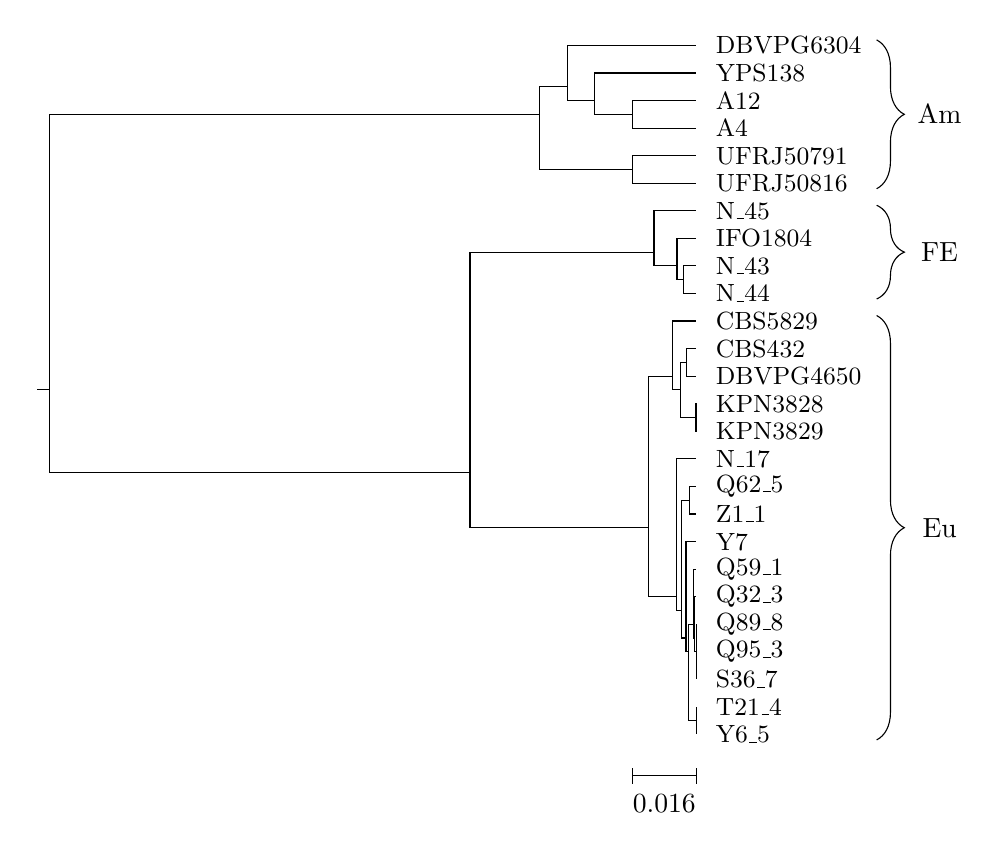
\begin{tikzpicture}[xscale=50,yscale=0.35]
    \node (r) at (0.0,0.0) {};
\node (rr) at (-0.0032859843,0.0) {};
\draw (r.center) -- (rr.center);
\node (r1) at (0.124339595,10.0) {};
\node (r11) at (0.1315726,11.0) {};
\node[label={[font=\small]right:DBVPG6304}] (r111) at (0.16429922,12.5) {};
\draw (r11.center) |- (r111.center);
\node (r112) at (0.13834648,10.5) {};
\node[label={[font=\small]right:YPS138}] (r1121) at (0.16429923,11.5) {};
\draw (r112.center) |- (r1121.center);
\node (r1122) at (0.14807872,10.0) {};
\node[label={[font=\small]right:A12}] (r11221) at (0.16429922,10.5) {};
\draw (r1122.center) |- (r11221.center);
\node[label={[font=\small]right:A4}] (r11222) at (0.16429922,9.5) {};
\draw (r1122.center) |- (r11222.center);
\draw (r112.center) |- (r1122.center);
\draw (r11.center) |- (r112.center);
\draw (r1.center) |- (r11.center);
\node (r12) at (0.14807872,8.0) {};
\node[label={[font=\small]right:UFRJ50791}] (r121) at (0.16429922,8.5) {};
\draw (r12.center) |- (r121.center);
\node[label={[font=\small]right:UFRJ50816}] (r122) at (0.16429922,7.5) {};
\draw (r12.center) |- (r122.center);
\draw (r1.center) |- (r12.center);
\draw (r.center) |- (r1.center);
\node (r2) at (0.106791504,-3.0) {};
\node (r21) at (0.15354072,5.0) {};
\node[label={[font=\small]right:N\_45}] (r211) at (0.16429922,6.5) {};
\draw (r21.center) |- (r211.center);
\node (r212) at (0.15938796,4.5) {};
\node[label={[font=\small]right:IFO1804}] (r2121) at (0.1642992,5.5) {};
\draw (r212.center) |- (r2121.center);
\node (r2122) at (0.16096471,4.0) {};
\node[label={[font=\small]right:N\_43}] (r21221) at (0.16429922,4.5) {};
\draw (r2122.center) |- (r21221.center);
\node[label={[font=\small]right:N\_44}] (r21222) at (0.16429922,3.5) {};
\draw (r2122.center) |- (r21222.center);
\draw (r212.center) |- (r2122.center);
\draw (r21.center) |- (r212.center);
\draw (r2.center) |- (r21.center);
\node (r22) at (0.15209067,-5.0) {};
\node (r221) at (0.15820873,0.5) {};
\node[label={[font=\small]right:CBS5829}] (r2211) at (0.16429923,2.5) {};
\draw (r221.center) |- (r2211.center);
\node (r2212) at (0.16037111,0.0) {};
\node (r22121) at (0.16173123,1.0) {};
\node[label={[font=\small]right:CBS432}] (r221211) at (0.16429923,1.5) {};
\draw (r22121.center) |- (r221211.center);
\node[label={[font=\small]right:DBVPG4650}] (r221212) at (0.16429923,0.5) {};
\draw (r22121.center) |- (r221212.center);
\draw (r2212.center) |- (r22121.center);
\node (r22122) at (0.16422524,-1.0) {};
\node[label={[font=\small]right:KPN3828}] (r221221) at (0.16429923,-0.5) {};
\draw (r22122.center) |- (r221221.center);
\node[label={[font=\small]right:KPN3829}] (r221222) at (0.16429923,-1.5) {};
\draw (r22122.center) |- (r221222.center);
\draw (r2212.center) |- (r22122.center);
\draw (r221.center) |- (r2212.center);
\draw (r22.center) |- (r221.center);
\node (r222) at (0.15933868,-7.5) {};
\node[label={[font=\small]right:N\_17}] (r2221) at (0.16429923,-2.5) {};
\draw (r222.center) |- (r2221.center);
\node (r2222) at (0.16052471,-8.0) {};
\node (r22221) at (0.16261172,-4.0) {};
\node[label={[font=\small]right:Q62\_5}] (r222211) at (0.16429922,-3.5) {};
\draw (r22221.center) |- (r222211.center);
\node[label={[font=\small]right:Z1\_1}] (r222212) at (0.16429922,-4.5) {};
\draw (r22221.center) |- (r222212.center);
\draw (r2222.center) |- (r22221.center);
\node (r22222) at (0.1616616,-9.0) {};
\node[label={[font=\small]right:Y7}] (r222221) at (0.16429922,-5.5) {};
\draw (r22222.center) |- (r222221.center);
\node (r222222) at (0.16238672,-9.5) {};
\node (r2222221) at (0.16348071,-8.5) {};
\node[label={[font=\small]right:Q59\_1}] (r22222211) at (0.16429922,-6.5) {};
\draw (r2222221.center) |- (r22222211.center);
\node (r22222212) at (0.16382422,-9.0) {};
\node[label={[font=\small]right:Q32\_3}] (r222222121) at (0.16429922,-7.5) {};
\draw (r22222212.center) |- (r222222121.center);
\node (r222222122) at (0.16429922,-9.5) {};
\node[label={[font=\small]right:Q89\_8}] (r2222221221) at (0.16429922,-8.5) {};
\draw (r222222122.center) |- (r2222221221.center);
\node[label={[font=\small]right:Q95\_3}] (r2222221222) at (0.16429922,-9.5) {};
\draw (r222222122.center) |- (r2222221222.center);
\node[label={[font=\small]right:S36\_7}] (r2222221223) at (0.16429922,-10.5) {};
\draw (r222222122.center) |- (r2222221223.center);
\draw (r22222212.center) |- (r222222122.center);
\draw (r2222221.center) |- (r22222212.center);
\draw (r222222.center) |- (r2222221.center);
\node (r2222222) at (0.16429922,-12.0) {};
\node[label={[font=\small]right:T21\_4}] (r22222221) at (0.16429922,-11.5) {};
\draw (r2222222.center) |- (r22222221.center);
\node[label={[font=\small]right:Y6\_5}] (r22222222) at (0.16429922,-12.5) {};
\draw (r2222222.center) |- (r22222222.center);
\draw (r222222.center) |- (r2222222.center);
\draw (r22222.center) |- (r222222.center);
\draw (r2222.center) |- (r22222.center);
\draw (r222.center) |- (r2222.center);
\draw (r22.center) |- (r222.center);
\draw (r2.center) |- (r22.center);
\draw (r.center) |- (r2.center);
\draw[|-|] (0.16429922,-14.0) -- (0.14786929,-14.0);
\node at (0.15608425,-15.0) {0.016};

\draw [decorate,decoration={brace,amplitude=10pt}]
(0.21, 12.7) -- (0.21, 7.3) node [black,midway,xshift=0.8cm] {Am};

\draw [decorate,decoration={brace,amplitude=10pt}]
(0.21, 6.7) -- (0.21, 3.3) node [black,midway,xshift=0.8cm] {FE};

\draw [decorate,decoration={brace,amplitude=10pt}]
(0.21, 2.7) -- (0.21, -12.7) node [black,midway,xshift=0.8cm] {Eu};

  \end{tikzpicture}
  \endpgfgraphicnamed
  \caption{An equidistant tree returned by \textsc{Lasso} from the yeast
    dataset with $10\%$ of the distances randomly removed. The sixteen
    European strains are denoted by the label ``Eu'', the four Far Eastern
    strains by ``FE'' and the six American strains by ``Am''. The uppermost
    five European strains (CBS5829 to KPN3829), together with N\_17, derive
    from outside the UK, with the remaining ten European strains having been
    isolated within the UK.}
  \label{fig:yeast-tree-complete}
\end{figure}

Since \textsc{Lasso}'s ability to reconstruct an equidistant tree from a
partial distance depends on both which distances are missing and the random
decisions made by the algorithm to break ties, we also constructed a consensus
tree from the equidistant trees returned by \textsc{Lasso} (see
Figure~\ref{fig:yeast-tree-consense}).  For this, we used an approach similar
to bootstrapping and indicate in terms of numbers assigned to each internal
vertex, except the root, how often each cluster induced by such a vertex is
displayed by an equidistant tree returned by \textsc{Lasso}.  More precisely
we generated 100 partial distances with $10\%$ of the distances removed at
random as described above.  We then ran \textsc{Lasso} on each partial
distance resulting in a total of $100$ equidistant trees each supported, on
average, by a strong lasso with 205 cords (out of the possible 293).  The
resulting trees were then used as input to the \textsc{Consense} program
\cite{felsenstein1993phylip} with default settings to build a consensus tree
using the ``majority rule (extended)" option. This tree is again highly
consistent with the full distance matrix tree, differing only from
Figure~\ref{fig:yeast-tree-complete} in the relationship between the three
European strains Q89\_8, Q95\_3 and S36\_7. Noticeably, the support for the
bifurcation of the latter two strains is the only one in
Figure~\ref{fig:yeast-tree-consense} less than 74.

\begin{figure}[t]
  \figureversion{lf}\tbfigures
  \centering
  \beginpgfgraphicnamed{yeast-tree-consense}
  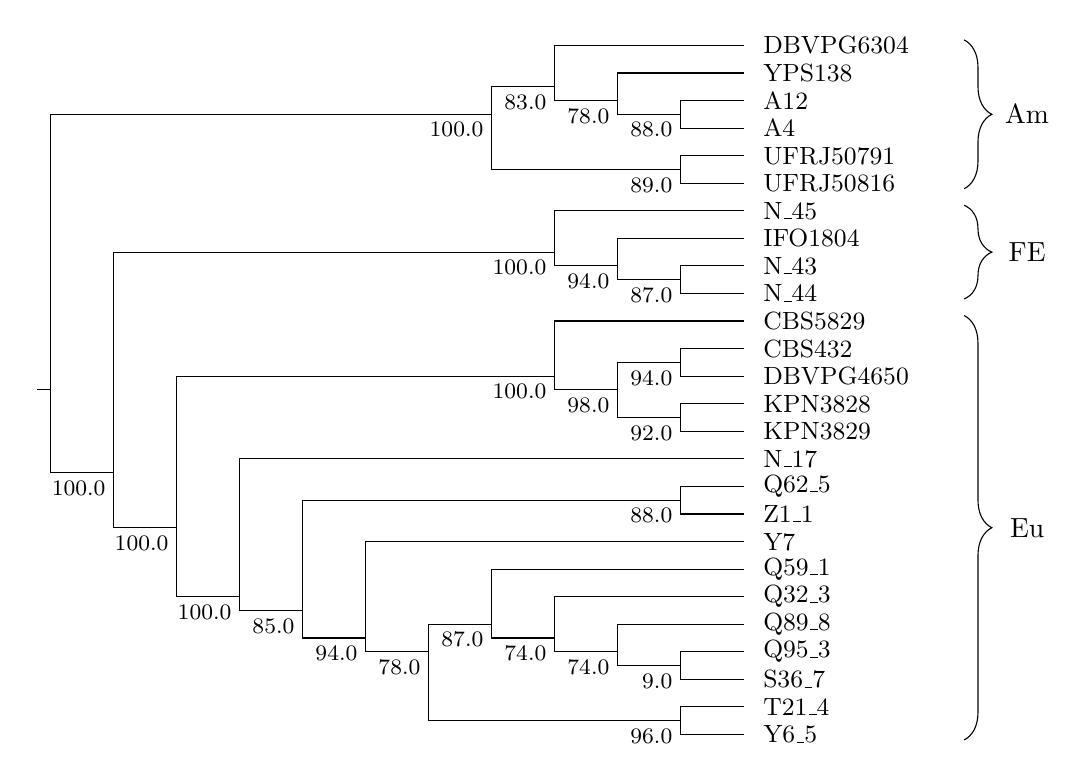
\begin{tikzpicture}[xscale=0.8,yscale=0.35]
    \node (r) at (0.0,0.0) {};
\node (rr) at (-0.22,0.0) {};
\draw (r.center) -- (rr.center);
\node[label={[label distance=-.2cm,font=\footnotesize]below left:100.0}] (r1) at (7.0,10.0) {};
\node[label={[label distance=-.2cm,font=\footnotesize]below left:83.0}] (r11) at (8.0,11.0) {};
\node[label={[font=\small]right:DBVPG6304}] (r111) at (11.0,12.5) {};
\draw (r11.center) |- (r111.center);
\node[label={[label distance=-.2cm,font=\footnotesize]below left:78.0}] (r112) at (9.0,10.5) {};
\node[label={[font=\small]right:YPS138}] (r1121) at (11.0,11.5) {};
\draw (r112.center) |- (r1121.center);
\node[label={[label distance=-.2cm,font=\footnotesize]below left:88.0}] (r1122) at (10.0,10.0) {};
\node[label={[font=\small]right:A12}] (r11221) at (11.0,10.5) {};
\draw (r1122.center) |- (r11221.center);
\node[label={[font=\small]right:A4}] (r11222) at (11.0,9.5) {};
\draw (r1122.center) |- (r11222.center);
\draw (r112.center) |- (r1122.center);
\draw (r11.center) |- (r112.center);
\draw (r1.center) |- (r11.center);
\node[label={[label distance=-.2cm,font=\footnotesize]below left:89.0}] (r12) at (10.0,8.0) {};
\node[label={[font=\small]right:UFRJ50791}] (r121) at (11.0,8.5) {};
\draw (r12.center) |- (r121.center);
\node[label={[font=\small]right:UFRJ50816}] (r122) at (11.0,7.5) {};
\draw (r12.center) |- (r122.center);
\draw (r1.center) |- (r12.center);
\draw (r.center) |- (r1.center);
\node[label={[label distance=-.2cm,font=\footnotesize]below left:100.0}] (r2) at (1.0,-3.0) {};
\node[label={[label distance=-.2cm,font=\footnotesize]below left:100.0}] (r21) at (8.0,5.0) {};
\node[label={[font=\small]right:N\_45}] (r211) at (11.0,6.5) {};
\draw (r21.center) |- (r211.center);
\node[label={[label distance=-.2cm,font=\footnotesize]below left:94.0}] (r212) at (9.0,4.5) {};
\node[label={[font=\small]right:IFO1804}] (r2121) at (11.0,5.5) {};
\draw (r212.center) |- (r2121.center);
\node[label={[label distance=-.2cm,font=\footnotesize]below left:87.0}] (r2122) at (10.0,4.0) {};
\node[label={[font=\small]right:N\_43}] (r21221) at (11.0,4.5) {};
\draw (r2122.center) |- (r21221.center);
\node[label={[font=\small]right:N\_44}] (r21222) at (11.0,3.5) {};
\draw (r2122.center) |- (r21222.center);
\draw (r212.center) |- (r2122.center);
\draw (r21.center) |- (r212.center);
\draw (r2.center) |- (r21.center);
\node[label={[label distance=-.2cm,font=\footnotesize]below left:100.0}] (r22) at (2.0,-5.0) {};
\node[label={[label distance=-.2cm,font=\footnotesize]below left:100.0}] (r221) at (8.0,0.5) {};
\node[label={[font=\small]right:CBS5829}] (r2211) at (11.0,2.5) {};
\draw (r221.center) |- (r2211.center);
\node[label={[label distance=-.2cm,font=\footnotesize]below left:98.0}] (r2212) at (9.0,0.0) {};
\node[label={[label distance=-.2cm,font=\footnotesize]below left:94.0}] (r22121) at (10.0,1.0) {};
\node[label={[font=\small]right:CBS432}] (r221211) at (11.0,1.5) {};
\draw (r22121.center) |- (r221211.center);
\node[label={[font=\small]right:DBVPG4650}] (r221212) at (11.0,0.5) {};
\draw (r22121.center) |- (r221212.center);
\draw (r2212.center) |- (r22121.center);
\node[label={[label distance=-.2cm,font=\footnotesize]below left:92.0}] (r22122) at (10.0,-1.0) {};
\node[label={[font=\small]right:KPN3828}] (r221221) at (11.0,-0.5) {};
\draw (r22122.center) |- (r221221.center);
\node[label={[font=\small]right:KPN3829}] (r221222) at (11.0,-1.5) {};
\draw (r22122.center) |- (r221222.center);
\draw (r2212.center) |- (r22122.center);
\draw (r221.center) |- (r2212.center);
\draw (r22.center) |- (r221.center);
\node[label={[label distance=-.2cm,font=\footnotesize]below left:100.0}] (r222) at (3.0,-7.5) {};
\node[label={[font=\small]right:N\_17}] (r2221) at (11.0,-2.5) {};
\draw (r222.center) |- (r2221.center);
\node[label={[label distance=-.2cm,font=\footnotesize]below left:85.0}] (r2222) at (4.0,-8.0) {};
\node[label={[label distance=-.2cm,font=\footnotesize]below left:88.0}] (r22221) at (10.0,-4.0) {};
\node[label={[font=\small]right:Q62\_5}] (r222211) at (11.0,-3.5) {};
\draw (r22221.center) |- (r222211.center);
\node[label={[font=\small]right:Z1\_1}] (r222212) at (11.0,-4.5) {};
\draw (r22221.center) |- (r222212.center);
\draw (r2222.center) |- (r22221.center);
\node[label={[label distance=-.2cm,font=\footnotesize]below left:94.0}] (r22222) at (5.0,-9.0) {};
\node[label={[font=\small]right:Y7}] (r222221) at (11.0,-5.5) {};
\draw (r22222.center) |- (r222221.center);
\node[label={[label distance=-.2cm,font=\footnotesize]below left:78.0}] (r222222) at (6.0,-9.5) {};
\node[label={[label distance=-.2cm,font=\footnotesize]below left:87.0}] (r2222221) at (7.0,-8.5) {};
\node[label={[font=\small]right:Q59\_1}] (r22222211) at (11.0,-6.5) {};
\draw (r2222221.center) |- (r22222211.center);
\node[label={[label distance=-.2cm,font=\footnotesize]below left:74.0}] (r22222212) at (8.0,-9.0) {};
\node[label={[font=\small]right:Q32\_3}] (r222222121) at (11.0,-7.5) {};
\draw (r22222212.center) |- (r222222121.center);
\node[label={[label distance=-.2cm,font=\footnotesize]below left:74.0}] (r222222122) at (9.0,-9.5) {};
\node[label={[font=\small]right:Q89\_8}] (r2222221221) at (11.0,-8.5) {};
\draw (r222222122.center) |- (r2222221221.center);
\node[label={[label distance=-.2cm,font=\footnotesize]below left:9.0}] (r2222221222) at (10.0,-10.0) {};
\node[label={[font=\small]right:Q95\_3}] (r22222212221) at (11.0,-9.5) {};
\draw (r2222221222.center) |- (r22222212221.center);
\node[label={[font=\small]right:S36\_7}] (r22222212222) at (11.0,-10.5) {};
\draw (r2222221222.center) |- (r22222212222.center);
\draw (r222222122.center) |- (r2222221222.center);
\draw (r22222212.center) |- (r222222122.center);
\draw (r2222221.center) |- (r22222212.center);
\draw (r222222.center) |- (r2222221.center);
\node[label={[label distance=-.2cm,font=\footnotesize]below left:96.0}] (r2222222) at (10.0,-12.0) {};
\node[label={[font=\small]right:T21\_4}] (r22222221) at (11.0,-11.5) {};
\draw (r2222222.center) |- (r22222221.center);
\node[label={[font=\small]right:Y6\_5}] (r22222222) at (11.0,-12.5) {};
\draw (r2222222.center) |- (r22222222.center);
\draw (r222222.center) |- (r2222222.center);
\draw (r22222.center) |- (r222222.center);
\draw (r2222.center) |- (r22222.center);
\draw (r222.center) |- (r2222.center);
\draw (r22.center) |- (r222.center);
\draw (r2.center) |- (r22.center);
\draw (r.center) |- (r2.center);

\draw [decorate,decoration={brace,amplitude=10pt}]
(14.5, 12.7) -- (14.5, 7.3) node [black,midway,xshift=0.8cm] {Am};

\draw [decorate,decoration={brace,amplitude=10pt}]
(14.5, 6.7) -- (14.5, 3.3) node [black,midway,xshift=0.8cm] {FE};

\draw [decorate,decoration={brace,amplitude=10pt}]
(14.5, 2.7) -- (14.5, -12.7) node [black,midway,xshift=0.8cm] {Eu};

  \end{tikzpicture}
  \endpgfgraphicnamed
  \caption{Consensus tree built from 100 runs of \textsc{Lasso} on matrices
    with 10\% of the distances randomly removed.  The number next to a vertex
    shows the number of times the cluster induced by that vertex appeared in
    the input of \textsc{Consense}. The length of an edge is of no relevance.}
  \label{fig:yeast-tree-consense}
\end{figure}

\subsection{A wheat dataset}
\label{sec:wheat-dataset}

Next, we analysed two partially overlapping wheat genetic marker datasets in
order to evaluate the potential of \textsc{Lasso} as a supertree approach. The
first dataset (which we will refer to as dataset $A$) consisted of 57 NBS
(Nucleotide Binding Site) markers scored over 411 accessions, a subset of a
dataset developed within the GEDIFLUX EU Framework V project \cite{gediflux}
to assess genetic diversity over time across four major crops, including
wheat. The second dataset (which we will refer to as dataset $B$) consisted of
71 NBS markers scored over 118 accessions, a subset of a study comparing
genetic diversity within and between winter wheat accessions from Turkey,
Kazakhstan and Europe \cite{muge}, the latter comprising a small group of the
GEDIFLUX wheat accessions. Consequently, the two datasets share a common set
of 26 European winter wheat accessions, comprising 6.3\% and 22.0\% of their
accessions respectively. We will refer to this shared dataset as dataset $C$.

\begin{figure}[t]
  \centering
  \includegraphics[scale=1]{figures/lasso-construction/supp-gedi-groups.pdf}
  \caption{The \textsc{Lasso} tree for wheat dataset $A$ coloured according to
    the groupings found by ADMIXTURE.}
  \label{fig:lasso-wheat-a}
\end{figure}

\begin{figure}[t]
  \centering
  \includegraphics[scale=0.8]{figures/lasso-construction/supp-muge-groups.pdf}
  \caption{The \textsc{Lasso} tree for wheat dataset $B$ coloured according to
    the groupings found by ADMIXTURE.}
  \label{fig:lasso-wheat-b}
\end{figure} 

Equidistant trees were estimated for datasets A and B separately, using the
Modified Rogers measure \cite{reif} to calculate a distance matrix, followed
by tree construction with \textsc{Lasso}. For convenience, we denote the two
distance matrices as $d_A$ and $d_B$, where the index indicates the dataset to
which they refer. The resulting equidistant trees were found to be supported
by 77,577 (out of 84,255) and 6,844 (out of 6,903) distances from $d_A$ and
$d_B$ respectively, and are shown in Figures~\ref{fig:lasso-wheat-a} and
\ref{fig:lasso-wheat-b}.  We assessed the individual \textsc{Lasso} trees
according to population group data for the two datasets. In the original
analysis of dataset $B$ \cite{muge}, the model-based clustering method
STRUCTURE \cite{structure} was carried out to estimate the number of founder
populations underlying the dataset and the genetic contribution of each
population to each accession. We coloured branches of the \textsc{Lasso} tree
in Figure~\ref{fig:lasso-wheat-b} such that the colour of each branch
corresponded to the main population group to which the relevant accession
belonged.  For dataset A, we conducted our own population structure analysis,
here using the ADMIXTURE method \cite{admixture} with default parameter
values.  ADMIXTURE uses an identical genetic model to STRUCTURE, but a
different computational approach to optimise population parameters, rendering
it considerably faster to run.  The \textsc{Lasso} tree for dataset $A$,
coloured according to these groups, is shown in
Figure~\ref{fig:lasso-wheat-a}. For both datasets, we see that accessions
belonging to the same population group are largely clustered within the
equidistant trees. The large sizes of the two Lassos (encompassing 92.1\% and
99.1\% of distances within $d_A$ and $d_B$ respectively), together with the
consistency of population grouping across the equidistant trees, strongly
suggest the suitability of the \textsc{Lasso} approach in determining the
genetic relationships between accessions within both of these
datasets. Furthermore, we note the previous use of the \textsc{UPGMA} method
to analyse NBS markers for wheat accessions \cite{mantovani06nbs}.

To obtain a (partial) distance $D$ on the combined dataset of $411+118-26=503$
accessions we proceeded as follows. If $x$ and $y$ are accessions such that
one of them is contained in dataset $A\backslash C$ and the other in $A$ then
we put $D(x,y)=d_A(x,y)$. Similarly, if one of them is contained in dataset
$B\backslash C$ and the other in $B$ then we put $D(x,y)=d_B(x,y)$. For the
remaining case that both accessions are contained in the overlap we took the
mean, that is, we put $D(x,y)=d_A(x,y)+d_B(x,y))/2$ where $x$ and $y$ are the
accessions under consideration.  To mitigate against the fact that for some
accessions in $C$ the distance values $d_A(x,y)$ and $d_B(x,y)$ correlate more
strongly than for others we used the ratio $d_A(x,y)/d_B(x,y)$ to identify
outliers, which we subsequently removed from the analysis. For this, we
employed the distribution of these ratios and defined a distance value to be
an outlier if it is more than one interquartile range above the upper quartile
or one interquartile range below the lower quartile.

\begin{figure}
  \centering \makebox[\textwidth][c]{\includegraphics[width=1.15\textwidth,
    trim = 20mm 65mm 20mm 55mm, clip]{figures/lasso-construction/bigtree.pdf}}
  \caption{The equidistant supertree built by \textsc{Lasso} for the two wheat
    datasets. Accessions from the GEDIFLUX dataset ($A$) are indicated by
    green branches, those from the Turkish dataset ($B$) by blue branches,
    with the 26 accessions found in both datasets ($C$) indicated by red
    branches. Note that the shared accessions are spread across the supertree
    and that the tree contains all 503 input taxa.}
  \label{fig:wheat-supertree}
\end{figure}

In total, the distance matrix representing $D$ contained 90,814 entries (where
we exclude entries of the form $D(x,x)$ and only count entries of the form
$D(x,y)$ and $D(y,x)$ once) which equates to $28.1\%$ of the $126,253$
potential distance values of a distance matrix on $503$ taxa missing.  We then
used this distance as input for \textsc{Lasso} to obtain a supertree $T$ on
the combined dataset. We depict that supertree in (Figure~
\ref{fig:wheat-supertree}) and remark in passing that the tree contains all
503 input taxa and that the size of the strong lasso returned by
\textsc{Lasso} supporting $T$ is 89,642. Put differently, $T$ is the unique
equidistant tree that displays correctly 98.7\% of the 90,814 distance values
for $D$.

To better understand the relevance of the obtained supertree $T$ we tested it
with regards to consistency with the original distances on the two
datasets. In addition, we compared its topology against the supertree
generated by the modified \textsc{MinCutSupertree} approach
\cite{page02mincut}.  For the former, we performed Mantel tests between the
distance matrices derived from $d_A$ and $d_B$ and the distances displayed by
$T$.  The tests showed a positive correlation of $0.57$ and $0.47$,
respectively, with $p$-values for both being $0.0009990$. These results
indicate that $T$ displayed relationships between accessions within the two
datasets appropriately, including the overlapping accessions.

For the latter, we employed again the Robinson-Foulds distance. More
precisely, we used the equidistant trees $T_A$ and $T_B$ generated by
\textsc{Lasso} from the datasets $A$ and $B$, respectively, to generate a
supertree $S$ using the modified \textsc{MinCutSupertree} approach. This tree
we then restricted to each of the data sets $A$ and $B$ resulting in the trees
$S|_A$ and $S|_B$, respectively. Next, we restricted the topology $t$ of $T$
to the accessions in $A$ and in $B$, respectively, resulting in the trees
$t|_A$ and $t|_B$ (where the index indicates the data set). For these four
trees we computed the Robinson-Foulds distances between them and found that
$D_{RF}(T_A,S|_A)= 96>79= D_{RF}(T_A,t|_A)$ and that $D_{RF}(T_B,S|_B)=
384>322=D_{RF}(T_B,t|_B)$.  This suggests that the topology of the supertree
returned by \textsc{Lasso} is closer to that of the original trees on the two
datasets than the supertree constructed by the modified
\textsc{MinCutSupertree} approach, thus highlighting {\sc Lassos}'s potential
as a supertree method.

\section{Conclusion}
\label{sec:conclusion-lasso}

\textsc{In this chapter}, we have proposed the novel \textsc{Lasso} approach
both for distance-based phylogenetic tree reconstruction and supertree
construction.  \textsc{Lasso} is similar in spirit to \textsc{UPGMA} but takes
as input partial distances and aims to reconstruct a unique (in a well-defined
sense), equidistant tree by exploiting redundancy in a given distance matrix
rather than trying to estimate missing distance values as do approaches such
as \cite{criscuolo2008fastnj}. Given that equidistant trees can be exploited
as starting trees within a search of tree space, for sophisticated
phylogenetic methods such as Maximum Likelihood and Bayesian Inference
\cite{burbrink09molecular,bouckaert14beast}, \textsc{Lasso} might provide a
quick and promising way to extend these methods to data sets for which only
partial distance information is available. Such datasets might arise when, for
example, confidence in a distance value is low resulting in an exclusion of
that distance (and thus the taxa involved) from an analysis, or when combining
disparate but overlapping datasets in a supertree context.

We assessed the performance of \textsc{Lasso} by means of artificial and real
biological data.  For the former we considered three different types of binary
equidistant trees and found that, independent of the tree type, \textsc{Lasso}
showed great promise when up to approximately $10\%$ of distance values were
missing.  For higher percentages of missing distance values we found that the
type of equidistant tree started to affect our ability to accurately
reconstruct it. More precisely, the equidistant caterpillar tree was recovered
most accurately under our simulation scenario and the equidistant balanced
tree the least accurately, with the equidistant Yule-Harding tree faring
slightly better than the balanced tree.  We also found that \textsc{Lasso}
showed great promise when the (unknown) equidistant tree underlying the given
partial distance did not possess vertices of too high a degree if a high
proportion of distance values were missing.  Put another way, even with $10\%$
of distance values missing for an underlying equidistant tree with vertices of
maximal out-degree $10$, \textsc{Lasso} was still able to return a tree on
more than $80\%$ of the original taxa.

We also assessed the performance of \textsc{Lasso} on two real biological
datasets. In the first of these studies, a yeast dataset originally developed
and analysed in \cite{west14ribosomal} was successfully reconstructed by
\textsc{Lasso}, even with 10\% of distance values removed at random. In the
second study, \textsc{Lasso} was used to construct a supertree of two
partially overlapping wheat NBS marker datasets \cite{gediflux,
  muge}. Subsequent statistical tests showed both that the \textsc{Lasso}
supertree successfully displayed relationships found with the two original
datasets and that it was more consistent with the two underlying trees than a
supertree constructed using the rival modified \textsc{MinCutSupertree}
approach. Collectively, these studies suggest that \textsc{Lasso} is
potentially a highly useful method for both tree reconstruction and supertree
construction on real datasets.

It is interesting to speculate that the strong performance of \textsc{Lasso}
in a supertree context owes part of its success to its ability to reject
shared distances that are not highly correlated. Indeed, when we repeated our
Mantel tests comparing the equidistant supertree derived from the full
combined dataset (that is, not rejecting any shared distance values) to the
two separate distance matrices (A and B), the correlations were found to be
0.47 ($p = 0.0009990$) for both datasets. Although this performance is almost
identical for dataset $B$, we see that removing certain shared distances leads
to a highly improved result for dataset $A$, which we earlier noted possessed
a lower proportion of distance values within the \textsc{Lasso}.  In future,
an investigation of methods to combine datasets for supertree construction
would be highly valuable, to see whether a further improvement could be
obtained.

Additional future work might include updating the distance in each repetition
step in a different way.  An alternative might be to simply throw out outliers
and remain much more tolerant to non-ultrametric input.  Although as we become
more tolerant to this we are less able to claim that we are satisfying the
consistency property.  We decided to only remove distances to avoid the
problems that come with introducing distances that exist with other methods
(as in Section~\ref{sec:constr-from-part}), but it might also be worth
considering introducing distances under certain circumstances.  For example,
we may consider adding one distance if it would allow us to grow our suitable
clique further.  Also it might be interesting to investigate the
\textsc{Lasso} approach in a {\em relaxed} molecular clock framework
\cite{drummond06relaxed}.

In summary, we propose the \textsc{Lasso} approach to become a new method
within the molecular phylogenetics toolkit. Given its demonstrated potential
both in tree reconstruction in the face of missing data, and in supertree
construction, we believe it can play an important role within a key project of
our generation, uncovering the Tree of Life.

\section{Acknowledgements}
\label{sec:acknowledgements}

\textsc{For their assistance} in the preparation of the paper underlining this
chapter we gratefully acknowledge Lesley Boyd and Muge Sayar-Turet for
providing a wheat dataset and Andrei-Alin Popescu for help with the ADMIXTURE
analysis and testing of software.

%%% Local Variables:
%%% TeX-master: "thesis"
%%% End:
